% !TEX root = ../thesis.tex

For the final set of simulations, we have to introduce the Rankine-vortex.
It is an idealized model of a vortex, mixing the definitions of a rigid body vortex
with constant vorticity and a potential vortex which has infinite vorticity in its center and zero otherwise.

\begin{figure}
\centering
\begin{subfigure}[b]{.5\textwidth}
  \centering
  % !TEX root = ../../thesis.tex

\begin{tikzpicture}
  \begin{axis}[
  axis x line=center,
  axis y line=center,
  xtick={-5,-4,...,5},
  ytick={-1,-0.5,...,1},
  xmin=-5.5,
  xmax=6.5,
  ymin=-1.2,
  ymax=1.5,
  x post scale=1.6,
  y post scale=0.7,
  xlabel=$x$,
  ylabel=$u_y$,
  samples=200]
  \addplot[blue,domain=1:5] {1/x};
  \addplot[blue,domain=-5:-1] {1/x};
  \addplot[blue,domain=-1:1] {x};
  \end{axis}
\end{tikzpicture}

  \caption{$y$-velocity}
\label{fig: rankine}
\end{subfigure}%
\begin{subfigure}[b]{.5\textwidth}
  \centering
  % !TEX root = ../../thesis.tex

\begin{tikzpicture}
  \begin{axis}[
  axis x line=center,
  axis y line=center,
  xtick={-1,...,1},
  ytick={0,1},
  xmin=-5.5,
  xmax=6.5,
  ymin=-1.2,
  ymax=1.5,
  x post scale=1,
  y post scale=0.7,
  xlabel=$x$,
  ylabel=$vorticity$,
  samples=200]

  \addplot[blue,thick,domain=1:5] {0};
  \addplot[blue,thick,domain=-5:-1] {0};
  \addplot[blue,thick,domain=-1:1] {1};
  \addplot[color=blue, thick,dashed] coordinates {
                    (1, 0)
                    (1,1)
                };
  \addplot[color=blue, thick,dashed] coordinates {
                    (-1, 0)
                    (-1,1)
                };
  \fill [fill=white] (axis cs:-0.2,-2.2) rectangle (axis cs:0.2,-0.05);
  \node at (axis cs:0.01,-0.23) {$0$};
  \end{axis}
\end{tikzpicture}

  \caption{Vorticity}
\label{fig: rankine vorticity}
\end{subfigure}
\caption{Cut through the middle of a Rankine vortex.
The inner part is a rigid body vortex with constant vorticity, whereas the outer part is a potential vortex which is vorticity free in this area.}
\label{fig: rankine}
\end{figure}

Figure~\ref{fig: rankine} shows the $y$ component of the velocity when cutting through a Rankine vortex at $y=0$, the $x$ component is zero.
A more thorough description of the Rankine vortex can be found in~\cite{giaiotti2006rankine}.

\begin{figure}
  \centering
  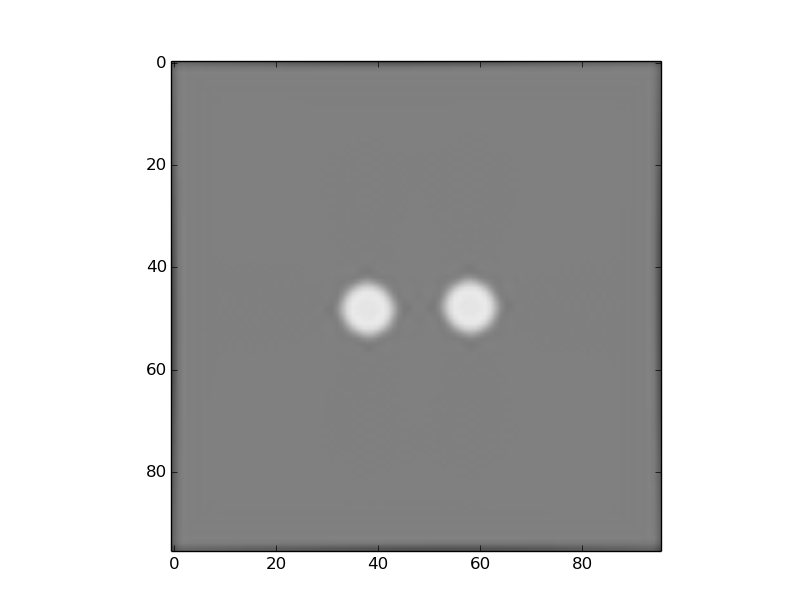
\includegraphics[width=0.6\textwidth]{../figures/rankine_vortex.png}  % chktex 11
  \caption{Setup for the vortex merge simulation on a $96^2$ grid. White is positive and black negative vorticity.}
\label{fig: vortex merge setup}
\end{figure}

The most simple nontrivial setting is depicted in Figure~\ref{fig: vortex merge setup} and consists of two vortices next to each other with the same direction of rotation, in our case conterclockwise, i.e.\ with positive vorticity.

\begin{figure}
\centering
\begin{subfigure}[b]{\textwidth}
  \centering
  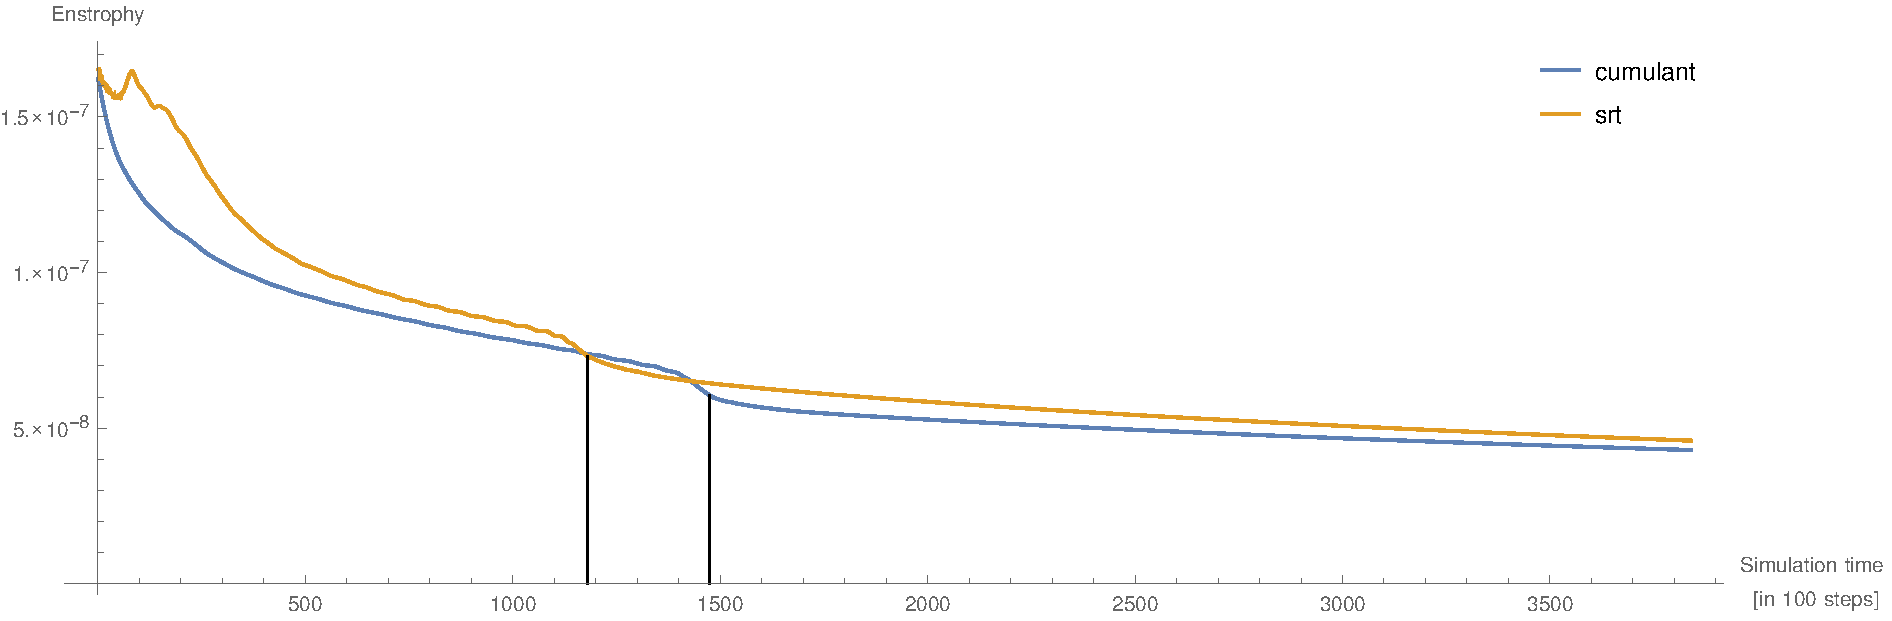
\includegraphics[width=\textwidth]{../figures/vortexMerge_enstrophy.pdf}  % chktex 11
  \caption{Evolution of the enstrophy}
\label{fig: rankine result}
\end{subfigure}%

\medskip
\begin{subfigure}[b]{.5\textwidth}
  \centering
  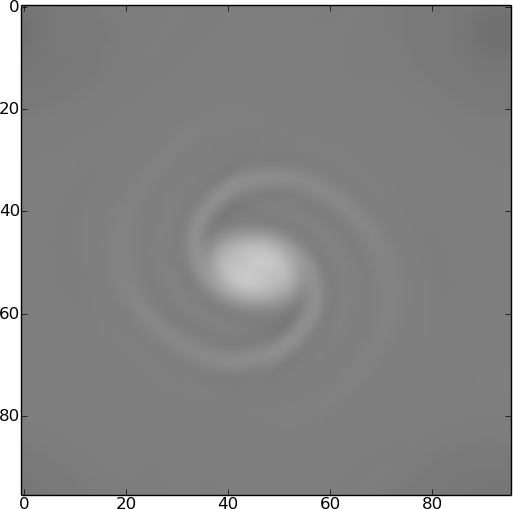
\includegraphics[width=0.6\textwidth]{../figures/cumulant_Re6000_size96_1475.png}  % chktex 11
  \caption{Simulation with cumulants at  $x=1475$}
\label{fig: rankine cumulant}
\end{subfigure}\begin{subfigure}[b]{.5\textwidth}
  \centering
  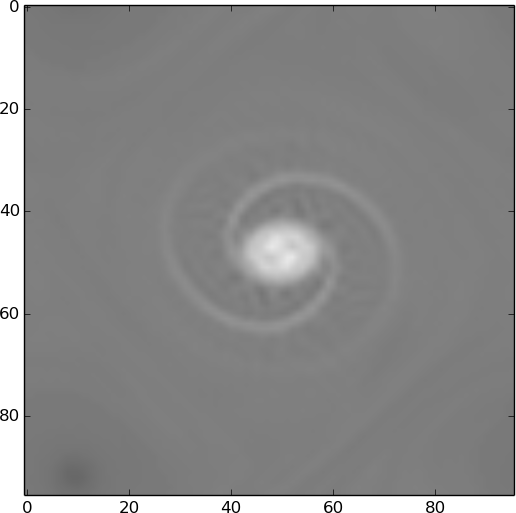
\includegraphics[width=0.6\textwidth]{../figures/srt_Re6000_size96_1181.png}  % chktex 11
  \caption{Simulation with \gls{srt} at  $x=1181$}
\label{fig: rankine srt}
\end{subfigure}

\caption{Simulation of the vortex merging at Reynolds number $6000$}
\label{fig: rankine 6000}
\end{figure}


\begin{figure}
\centering
\begin{subfigure}[b]{\textwidth}
  \centering
  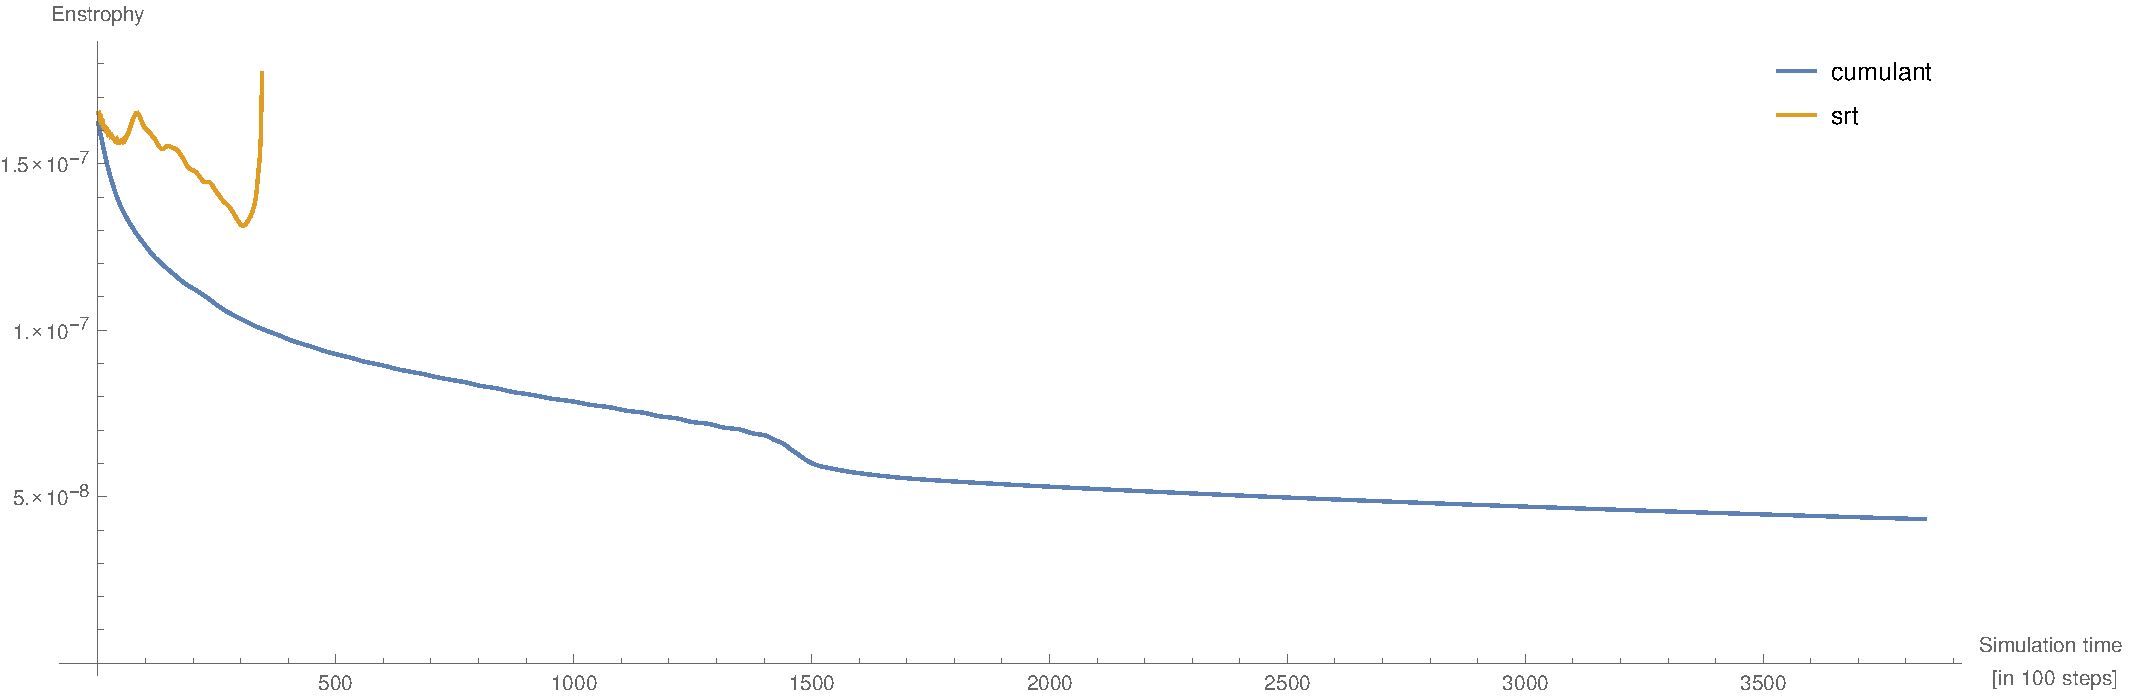
\includegraphics[width=\textwidth]{../figures/vortexMerge_enstrophy6100.pdf}  % chktex 11
  \caption{Evolution of the enstrophy at Reynolds number $6100$}
\label{fig: rankine 6000}
\end{subfigure}%

\medskip
\begin{subfigure}[b]{\textwidth}
  \centering
  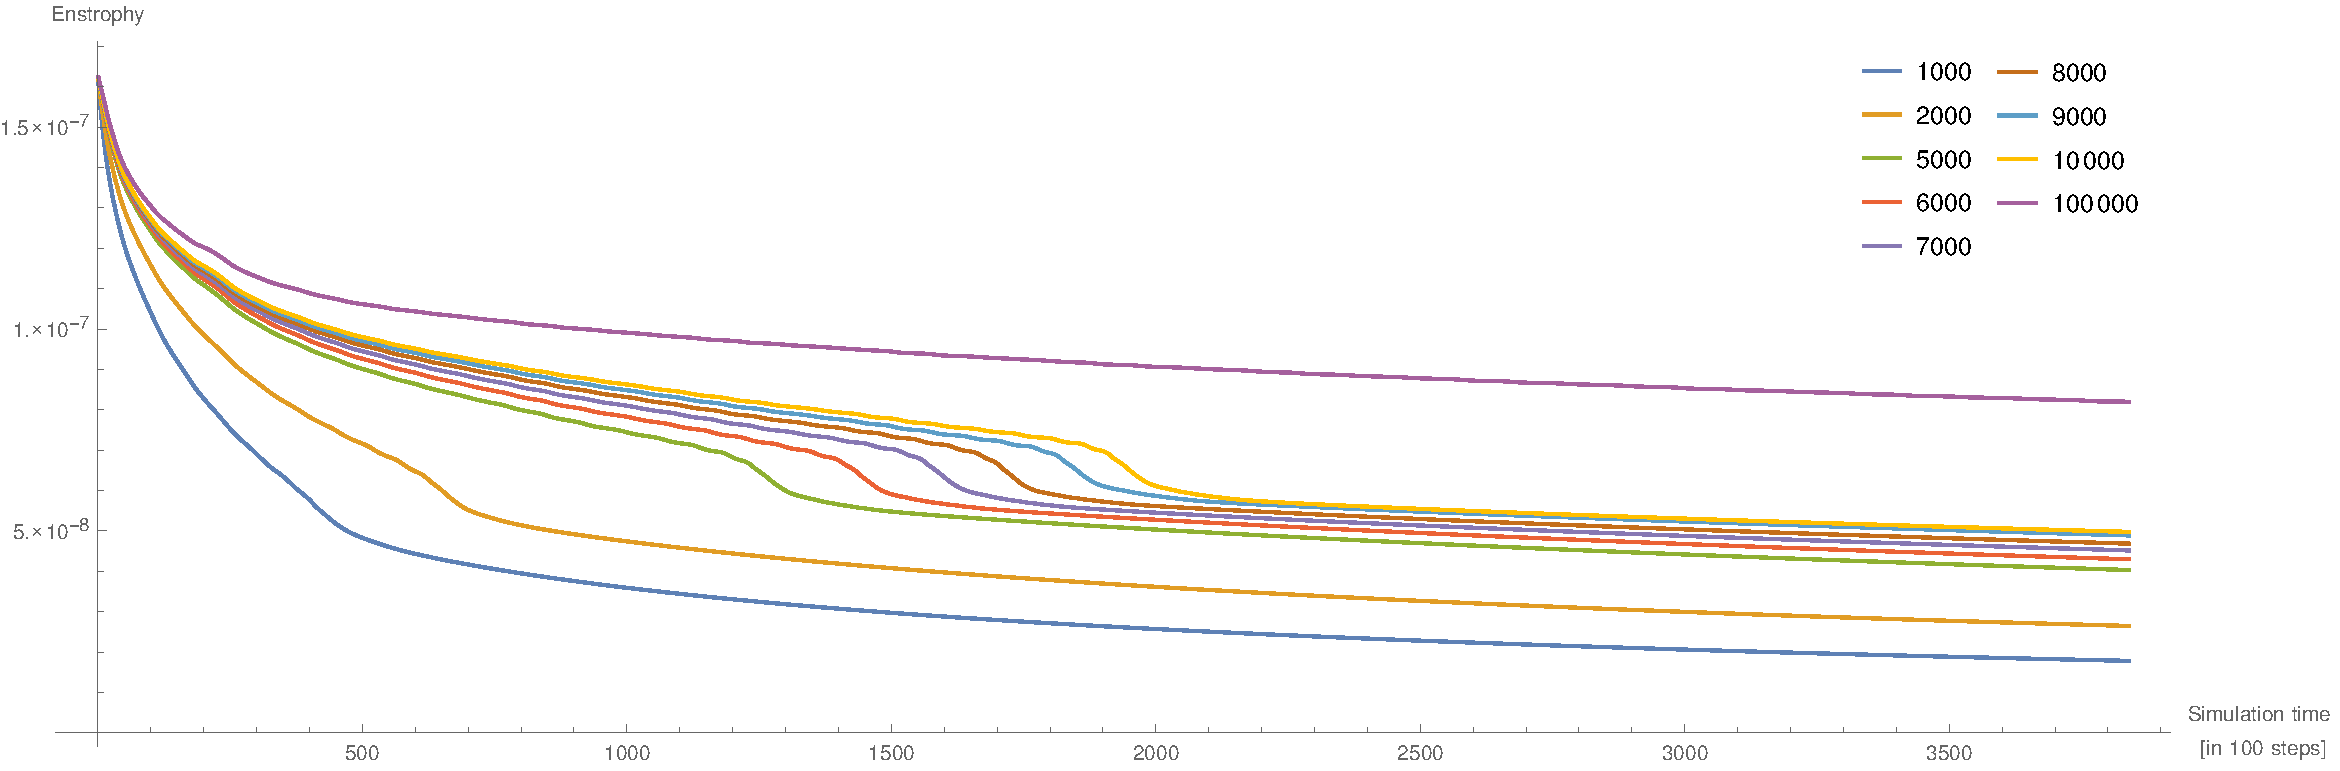
\includegraphics[width=\textwidth]{../figures/vortexMerge_enstrophy_cumulants.pdf}  % chktex 11
  \caption{Evolution of the enstrophy at increasing Reynolds numbers with cumulant \gls{lbm}}
\label{fig: rankine cumulant all}
\end{subfigure}
\caption{Further simulation results}
\label{fig: rankine further}
\end{figure}
